\section{实验}\label{numerical experiments}
本文使用训练完毕的地图特征与解码器进行推理并导出地图的顶点与面元数据,以网格格式对结果进行评估。对于网格中每一个被分配的体素,本文将其再次细分为$N \times N \times N$个部分,直接推理出其内部$N^3$个点的SDF值和语义信息。最终本文使用marching cubes\cite{marchingcubes}等值面提取算法提取出地图的所有顶点与表面,并将语义信息映射为顶点颜色。
\subsection{实验准备}
\subsubsection{数据集}
本文的方法在3个公开的户外激光雷达数据集上进行了定性和定量的测试:(1)人工合成的MaiCity数据集\cite{maicity},模拟使用64线无噪声激光雷达对城市场景扫描序列组成。(2)真实世界的Newer College数据集\cite{ncd},该数据集在牛津大学内使用手持激光雷达记录,具有厘米级测量噪声和大量运动失真。其地面数据使用地面扫描仪获得。两者均带有地面附近的Ground Truth网格数据用作评估。(3) KITTI\cite{KITTI}是目前最大的自动驾驶场景下的计算机视觉算法评测数据集,SemanticKITTI\cite{SemanticKITTI}为其点云数据标注了语义信息。其数据包括激光雷达与RGB-D数据流等,每一帧中出现多个车辆或行人,包含超过20种语义标签类型。
\subsubsection{评价指标}
\subsubsection{实现细节}
\subsection{模拟场景}
\subsection{真实场景}
\subsection{算法时间与内存占用}
% 本节分别使用鲲鲲内卷法,中中内卷法,伟伟内卷法进行时间比较。在3天内,让实验组和对照组分别在3天内写论文。鲲鲲卷卷法3天写出了一篇CVPR,中中卷卷法3天写出了一篇AAAI,对照组三天写出了一份10页报告,而伟伟卷卷法3天从黄铜上分到了白银。

% \begin{figure}[hb!]
%     \centering
%     \subfigure[目标检测]{
%     \begin{minipage}[t]{0.22\linewidth}
%     \centering
%     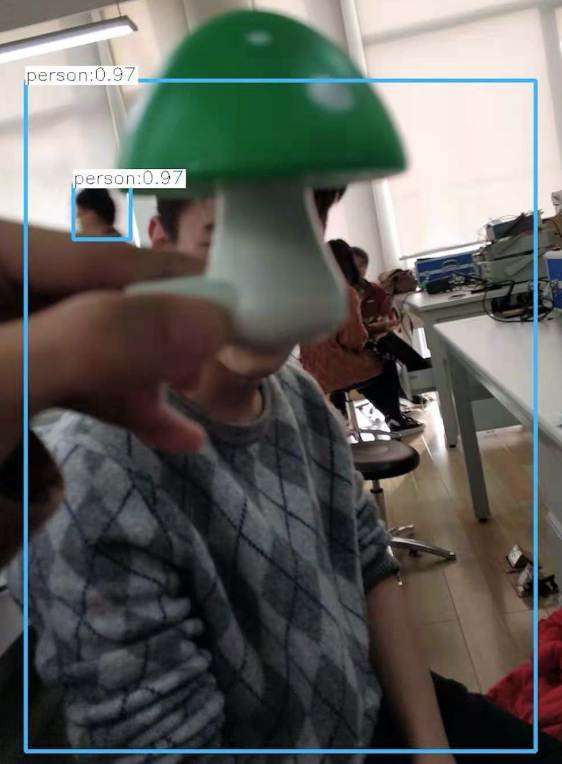
\includegraphics[width=\linewidth]{figures/det.png}
%     \end{minipage}\label{fig:det}
%     }
%     %
%     \centering
%     \subfigure[语义分割]{
%     \begin{minipage}[t]{0.28\linewidth}
%     \centering
%     
\includegraphics[width=\linewidth]{figures/seg.png}
%     \end{minipage}\label{fig:seg}
%     }
%     %
%     \centering
%     \subfigure[姿态识别]{
%     \begin{minipage}[t]{0.4\linewidth}
%     \centering
%     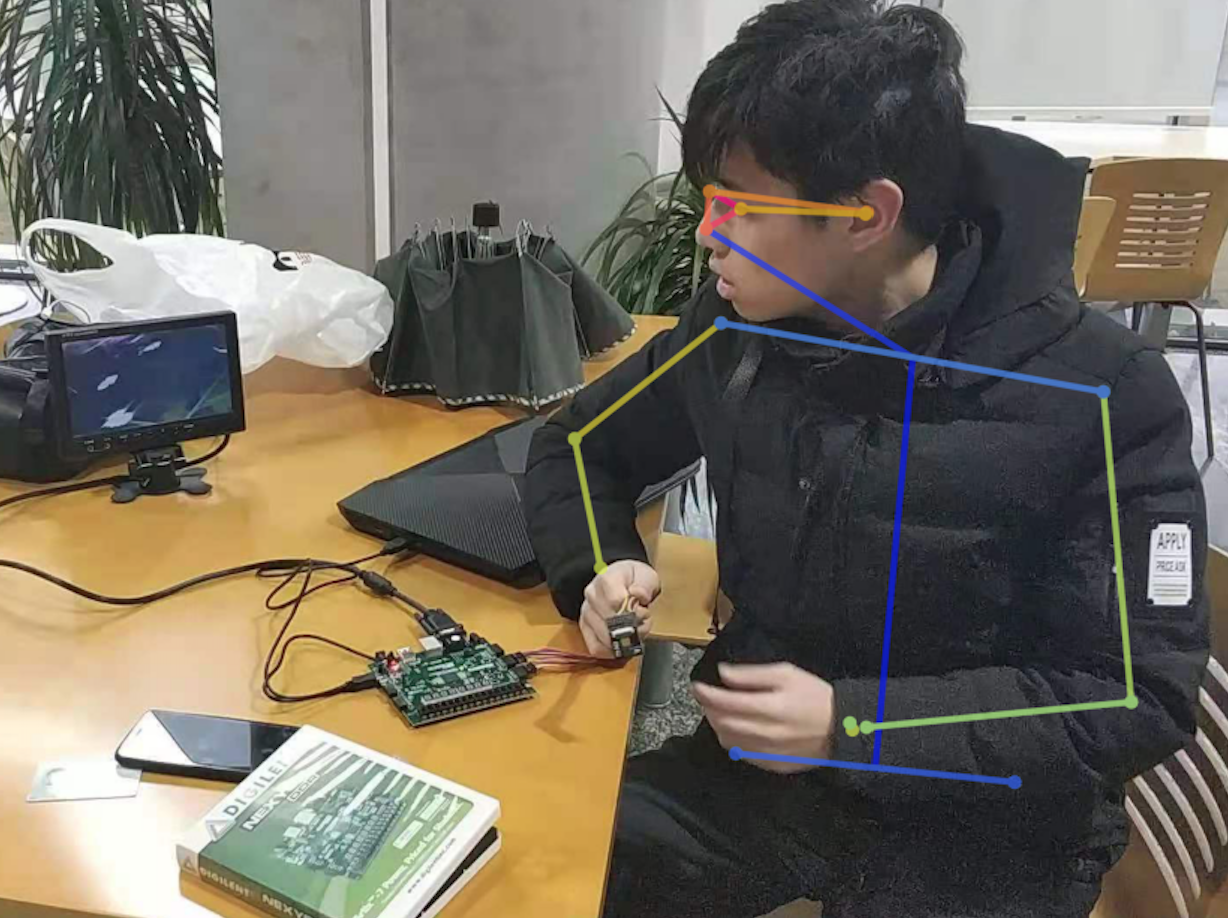
\includegraphics[width=\linewidth]{figures/pose.png}
%     \end{minipage}\label{fig:pose}
%     }
%     %
%     \caption{常见视频分析应用图解(图片提供者为中中同学)}\label{fig:cvexample}
%     \centering
% \end{figure}